\chapter[Resultados y validación]{Resultados y validación\label{cap:resultados}}

\section{Resultados experimentales}
\label{sec:results}

Este capítulo presenta los resultados obtenidos para los tres componentes
analíticos principales del prototipo: el agrupamiento automático de manchas
solares, la clasificación jerárquica Zurich--McIntosh y los modelos predictivos
de actividad solar. Más allá de la evaluación aislada de cada algoritmo, el
objetivo es analizar el comportamiento del sistema como una arquitectura
integrada orientada al registro y procesamiento asistido de observaciones
heliográficas. Esta organización es coherente con la estructura general del
trabajo descrita en el Capítulo 5 y con la validación integral del prototipo
presentada posteriormente. 

\subsection{Agrupamiento automático con YOLO26n}

En la etapa de agrupamiento, el detector basado en YOLO26n alcanzó una
precisión del orden del $83\%$ sobre el conjunto DB1, valor consistente con el
rango de desempeño reportado en la literatura para tareas equivalentes de
detección y agrupamiento de manchas solares en imágenes de disco completo.
Este resultado sugiere que el modelo logra identificar de forma robusta las
regiones activas relevantes y proporciona recortes suficientemente consistentes
para la etapa posterior de clasificación morfológica.

Debe señalarse que la evaluación de esta etapa no persigue una segmentación
pixel a pixel de umbra y penumbra, sino la delimitación espacial de regiones
activas como unidad observacional. Desde esta perspectiva, el rendimiento
obtenido se considera adecuado para el propósito del prototipo, ya que la
clasificación Zurich--McIntosh se aplica sobre grupos solares y no sobre manchas
aisladas.

\subsection{Clasificación jerárquica Zurich--McIntosh}

Antes de la comparación cuantitativa con trabajos de referencia, se analiza el
comportamiento probabilístico de la salida jerárquica propuesta. La
Figura~\ref{fig:resultados-arbol-top12-zpc} muestra el árbol bayesiano de
probabilidades para un caso representativo, donde la recomendación de clase no se
obtiene únicamente como una salida plana, sino como una combinación restringida
por la estructura válida de la taxonomía Zurich--McIntosh. 

\begin{figure}[H]
    \centering
    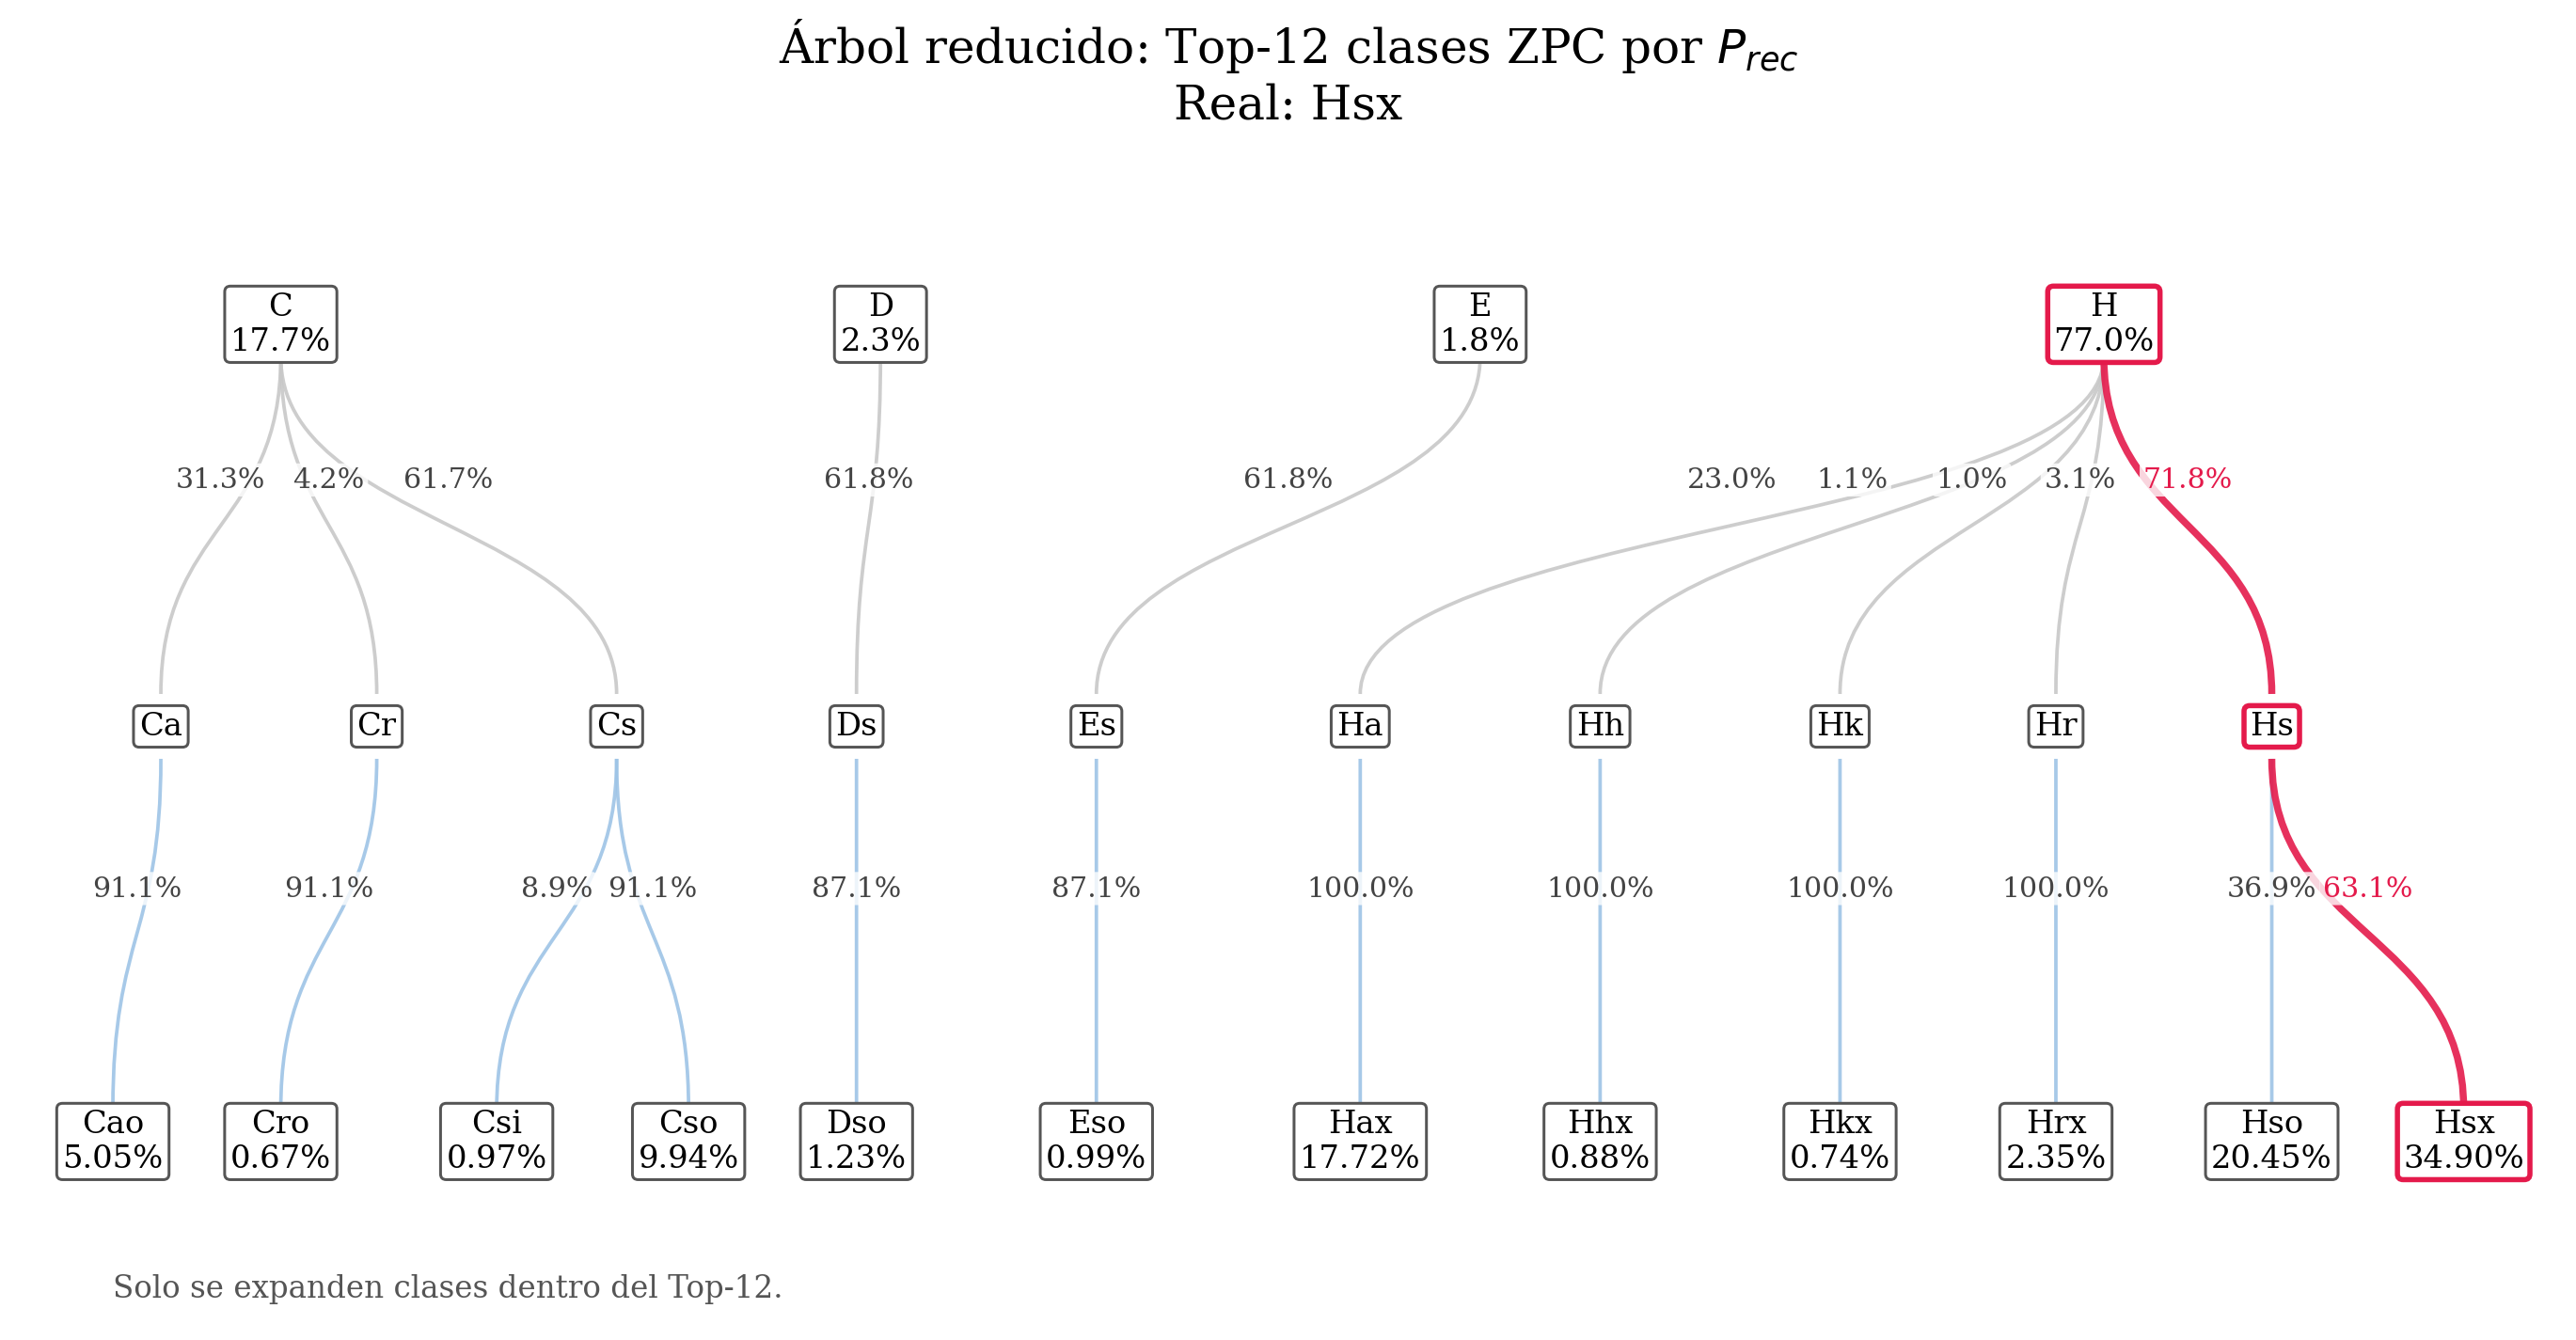
\includegraphics[width=0.92\textwidth]{figures/ml/top12_tree.png}
    \caption{Árbol bayesiano de probabilidades para la recomendación jerárquica
    Zurich--McIntosh. La visualización organiza las alternativas más probables
    según las componentes $Z$, $P$ y $C$, preservando la consistencia taxonómica
    de las clases válidas. \textbf{Fuente:} Elaboración propia.}
    \label{fig:resultados-arbol-top12-zpc}
\end{figure}

El árbol corresponde
a una implementación de los formalismos probabilísticos presentados en la
Sección~\ref{sec:classification}, donde la probabilidad conjunta se descompone de
forma jerárquica según las componentes $Z$, $P$ y $C$. Esta representación permite
inspeccionar cómo se distribuye la confianza desde el tipo de grupo $Z$ hacia las
componentes $P$ y $C$, y facilita identificar alternativas cercanas cuando existen
configuraciones morfológicamente similares.

La Figura~\ref{fig:resultados-top12-zpc} complementa esta lectura mediante un
histograma de las doce clases $ZPC$ con mayor probabilidad. El resultado muestra
que la masa probabilística se concentra en un subconjunto reducido de
combinaciones, mientras que las alternativas restantes presentan valores menores
pero todavía informativos. Este comportamiento es útil para un sistema de
asistencia observacional, ya que permite presentar una recomendación principal
junto con opciones secundarias ordenadas por plausibilidad, en lugar de forzar
una única etiqueta sin contexto de incertidumbre.

\begin{figure}[H]
    \centering
    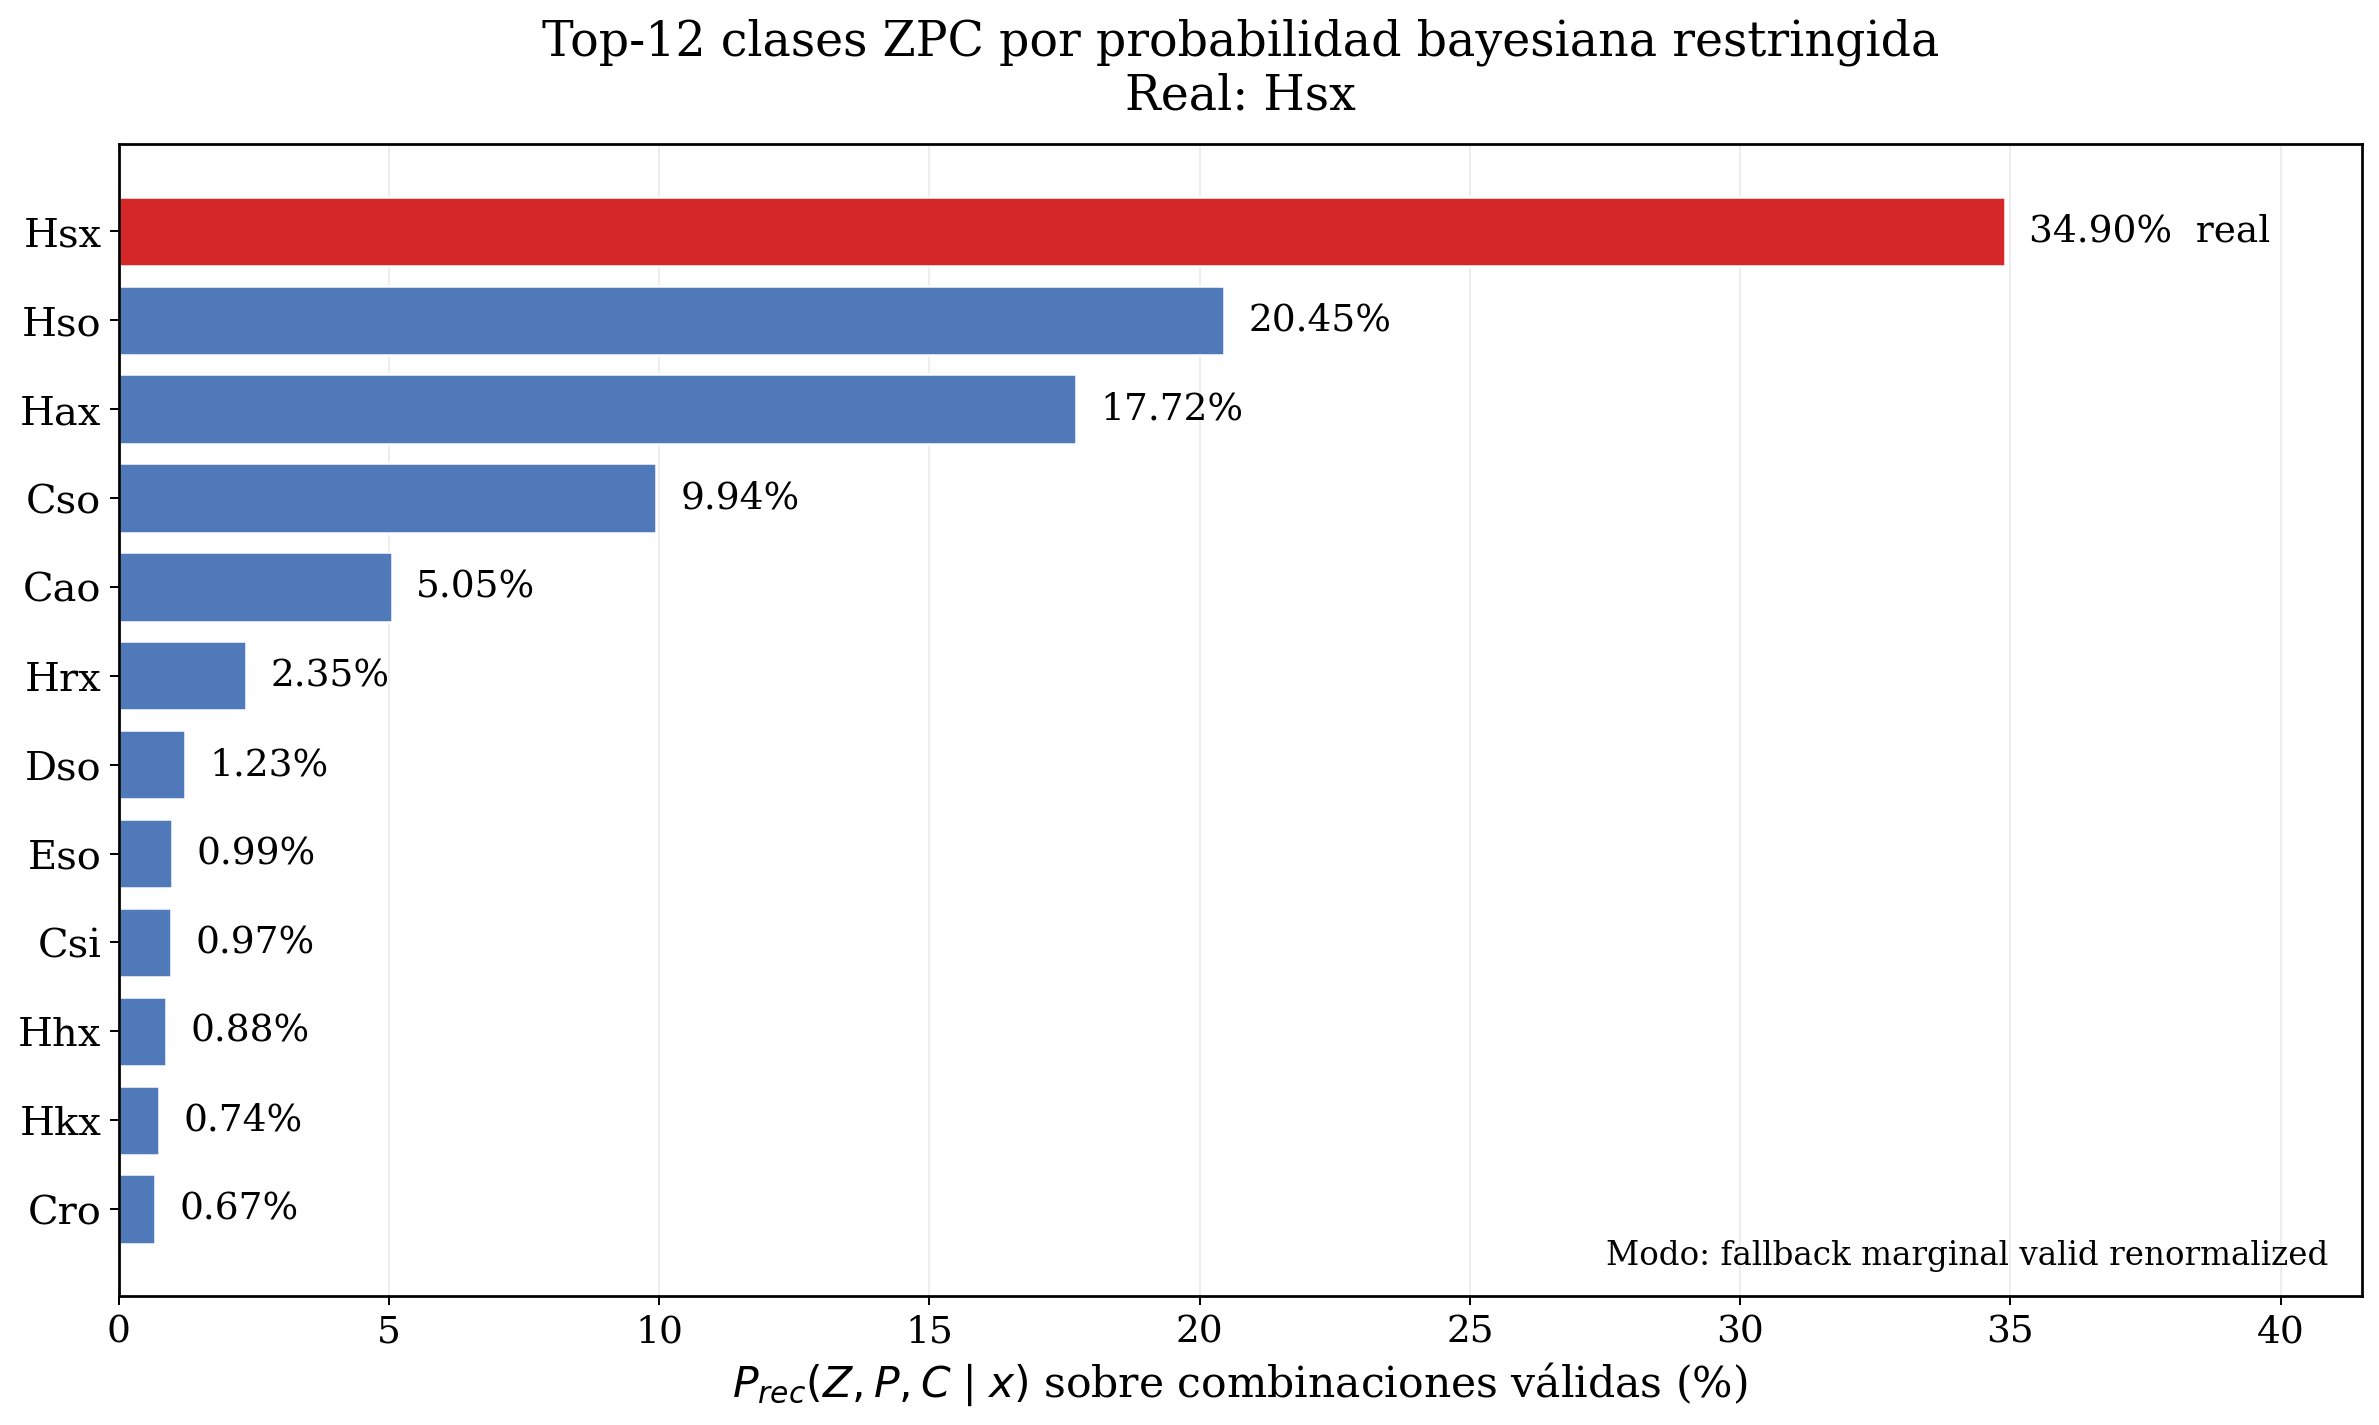
\includegraphics[width=0.92\textwidth]{figures/ml/top12_rec.png}
    \caption{Histograma del top 12 de clases Zurich--McIntosh recomendadas por
    probabilidad bayesiana restringida. La figura permite comparar la clase más
    probable con alternativas cercanas dentro del espacio válido de
    configuraciones $ZPC$. \textbf{Fuente:} Elaboración propia.}
    \label{fig:resultados-top12-zpc}
\end{figure}

Como síntesis comparativa, la Tabla~\ref{tab:comparativa-baselines} resume el
rendimiento por carácter bajo métrica F1 de trabajos representativos sobre
clasificación McIntosh, junto con la propuesta desarrollada en este manuscrito.

\begin{table}[H]
\centering
\caption{Comparación de F1-score para la clasificación McIntosh. Los valores
reportados se toman de las referencias correspondientes cuando están
disponibles. \textbf{Fuente:} Elaboración propia con base en la literatura citada.}
\label{tab:comparativa-baselines}
{\uniformtablestyle
\setlength{\tabcolsep}{7pt}
\begin{adjustbox}{center}
\begin{tabular}{lcccc}
\toprule
\textbf{Autor} & \textbf{F1-Z} & \textbf{F1-P} & \textbf{F1-C} & \textbf{F1 prom.} \\
\midrule
Palladino et al.\ (2022) \citep{palladino2022sunspot} & 0.67 & 0.55 & 0.72 & 0.65 \\
Sayez et al.\ (2023) \citep{sayez2023sunscc} & 0.68 & 0.65 & 0.72 & 0.68 \\
Deng et al.\ (2025) \citep{deng2025mcintosh} & 0.47 & 0.41 & 0.60 & 0.49 \\
Propuesta & 0.65 & 0.63 & 0.71 & 0.66 \\
\bottomrule
\end{tabular}
\end{adjustbox}
}
\end{table}

La propuesta alcanza un F1 promedio de $0.66$, valor próximo al mejor resultado
de referencia considerado en esta tesis ($0.68$). Esta comparación debe leerse
considerando la severidad de la métrica empleada: en este trabajo no se realiza
compactación artificial de clases ni se fusionan categorías raras para facilitar
la evaluación. Por el contrario, se conserva la taxonomía Zurich--McIntosh en sus
componentes originales, lo que obliga al modelo a distinguir diferencias sutiles
entre categorías cercanas, como $E$ y $F$ en la extensión longitudinal del grupo
o $C$ y $D$ en configuraciones bipolares compactas.

Desde esta perspectiva, mantener la granularidad taxonómica completa no se
considera una debilidad, sino una característica de diseño. Una clasificación
compactada podría elevar el F1 al reducir el número de fronteras difíciles, pero
también eliminaría información observacional útil para el usuario experto. La
propuesta privilegia una salida más estricta e interpretable, coherente con el
uso del sistema como herramienta de asistencia y revisión humana.

Más allá de los valores numéricos, las referencias comparadas responden a
decisiones metodológicas diferentes. Palladino et al.~\citep{palladino2022sunspot}
tratan cada componente ($Z$, $P$ y $C$) como un problema independiente.
Sayez et al.~\citep{sayez2023sunscc} proponen una arquitectura multitarea
jerárquica con ensamble y mecanismos adicionales de calibración de confianza.
Deng et al.~\citep{deng2025mcintosh} evalúan CNNs clásicas sobre particiones
más estrictas por región activa.

En contraste, la arquitectura desarrollada en esta tesis incorpora explícitamente
la dependencia jerárquica desde la salida $Z$ hacia las predicciones de $P$ y
$C$. Esta formulación preserva la semántica original de la taxonomía
Zurich--McIntosh y permite interpretar cada salida como una distribución de
probabilidad condicionada.

Los resultados también confirman que la componente $C$ es la de mejor
desempeño relativo, con un F1 de $0.71$, mientras que las mayores dificultades
se concentran en las componentes $Z$ y $P$, especialmente en clases con escaso
soporte muestral o fronteras morfológicas difusas. Este comportamiento es
consistente con las matrices de confusión analizadas en la Sección 5.2.2 y con
la distribución de cola larga observada en DB2.

En conjunto, estos resultados indican que la arquitectura jerárquica basada en
ConvNeXtV2 Atto logra un nivel de desempeño competitivo respecto al estado del
arte, manteniendo una estructura de salida interpretable y coherente con la
lógica observacional empleada por los catálogos Zurich--McIntosh. La elección de
la variante Atto respondió además a un criterio de despliegue: su tamaño reducido
favorece una conversión íntegra desde PyTorch hacia ONNX y facilita la ejecución
en entornos con recursos limitados. Las etapas MLP complementarias conservan el
aprendizaje jerárquico entre $Z$, $P$ y $C$ sin sacrificar la portabilidad de
las salidas.


\subsection{Resultados de los modelos predictivos}

La evaluación de los modelos predictivos se organiza en dos niveles complementarios. El primero corresponde al seguimiento escalar del número de manchas solares suavizado, denotado en la Sección~\ref{sec:forecast} como $\mathrm{SSN}_{\mathrm{PVLK}}(t_k)=\widehat{s}_k$, donde $\widehat{s}_k$ representa la estimación corregida del estado en el instante mensual $t_k$. El segundo corresponde a la reconstrucción espacio-temporal de la actividad latitudinal mediante DMD, donde el diagrama de Spörer se modela como una matriz de instantáneas $\mathbf{X}$ y su reconstrucción se denota por $\widehat{\mathbf{X}}$. Esta separación permite distinguir entre precisión de amplitud del ciclo y fidelidad en la migración latitudinal de la actividad.

Para la evaluación escalar se considera una secuencia observada $z_k$, asociada al SSN mensual suavizado, y una secuencia estimada $\widehat{s}_k$ generada por cada modelo en los mismos instantes $t_k$, con $k=1,\ldots,N$. A partir de estas dos series se calculan métricas de error absoluto, error cuadrático, error porcentual, ajuste global y correlación lineal. El error absoluto medio se define como
\begin{equation}
\mathrm{MAE}=\frac{1}{N}\sum_{k=1}^{N}\left|z_k-\widehat{s}_k\right|.
\end{equation}

La raíz del error cuadrático medio se calcula mediante
\begin{equation}
\mathrm{RMSE}=\sqrt{\frac{1}{N}\sum_{k=1}^{N}\left(z_k-\widehat{s}_k\right)^2}.
\end{equation}

El error porcentual absoluto medio se expresa como
\begin{equation}
\mathrm{MAPE}=\frac{100}{N}\sum_{k=1}^{N}\left|\frac{z_k-\widehat{s}_k}{z_k}\right|,
\end{equation}
siempre que $z_k\neq 0$ para los instantes considerados. El coeficiente de determinación se define como
\begin{equation}
R^2=1-\frac{\sum_{k=1}^{N}\left(z_k-\widehat{s}_k\right)^2}{\sum_{k=1}^{N}\left(z_k-\bar{z}\right)^2},
\end{equation}
donde $\bar{z}$ representa el promedio de la serie observada. Finalmente, la correlación de Pearson entre la serie observada y la estimada queda dada por
\begin{equation}
\rho=\frac{\sum_{k=1}^{N}\left(z_k-\bar{z}\right)\left(\widehat{s}_k-\bar{\widehat{s}}\right)}{\sqrt{\sum_{k=1}^{N}\left(z_k-\bar{z}\right)^2}\sqrt{\sum_{k=1}^{N}\left(\widehat{s}_k-\bar{\widehat{s}}\right)^2}},
\end{equation}
donde $\bar{\widehat{s}}$ es el promedio de la serie estimada.

Los resultados obtenidos para el periodo histórico se resumen en la Tabla~\ref{tab:ssn-metrics-comparison}. El modelo PVL--Kalman presenta el menor error absoluto y cuadrático, así como el mayor valor de $R^2$ y de correlación de Pearson. Esto indica que su formulación recursiva resulta particularmente adecuada para seguir la amplitud global del ciclo cuando el objetivo es aproximar la evolución temporal del SSN suavizado.

\begin{table}[H]
\centering
\caption{Comparativa de métricas de rendimiento para la predicción de SSN. \textbf{Fuente:} Elaboración propia basada en \texttt{ssn\_metrics.csv}.}
\label{tab:ssn-metrics-comparison}
\begin{tabular}{lccccc}
\hline
\textbf{Modelo} & \textbf{MAE} & \textbf{RMSE} & \textbf{MAPE (\%)} & \textbf{$R^2$} & \textbf{Pearson} \\ \hline
PVL--Kalman ($\mathrm{SSN}_{\mathrm{PVLK}}$) & 18.42 & 24.15 & 27.0 & 0.8942 & 0.9481 \\
DMD integral ($\mathrm{SSN}_{\mathrm{DMD}}$) & 22.15 & 29.84 & 33.0 & 0.8125 & 0.9104 \\ \hline
\end{tabular}
\end{table}

La evaluación del modelo DMD requiere métricas adicionales, porque su salida principal no es únicamente una serie escalar, sino una reconstrucción de la distribución latitudinal de la actividad. En este caso, $\mathbf{X}\in\mathbb{R}^{m\times N}$ representa la matriz observada de actividad latitudinal, donde cada columna corresponde a una instantánea mensual del diagrama de Spörer, y $\widehat{\mathbf{X}}$ representa la reconstrucción obtenida a partir del operador dinámico estimado. El error relativo de Frobenius se define como
\begin{equation}
E_F=\frac{\left\|\mathbf{X}-\widehat{\mathbf{X}}\right\|_F}{\left\|\mathbf{X}\right\|_F}.
\end{equation}

La coherencia espacio-temporal se evalúa mediante la correlación entre las matrices vectorizadas:
\begin{equation}
\rho_{ST}=\mathrm{corr}\left(\mathrm{vec}(\mathbf{X}),\mathrm{vec}(\widehat{\mathbf{X}})\right).
\end{equation}

Para medir la coherencia de la migración latitudinal se utiliza el error medio del centro latitudinal de actividad. Si $\theta_{c,k}$ es el centro latitudinal observado en el instante $t_k$ y $\widehat{\theta}_{c,k}$ su estimación reconstruida, entonces
\begin{equation}
\mathrm{MLCE}=\frac{1}{N}\sum_{k=1}^{N}\left|\theta_{c,k}-\widehat{\theta}_{c,k}\right|.
\end{equation}

La Tabla~\ref{tab:sporer-performance} resume los indicadores asociados a la reconstrucción latitudinal.

\begin{table}[H]
\centering
\caption{Métricas de reconstrucción espacio-temporal mediante DMD. \textbf{Fuente:} Elaboración propia basada en \texttt{sporer\_metrics.csv}.}
\label{tab:sporer-performance}
\begin{tabular}{lc}
\hline
\textbf{Métrica} & \textbf{Valor observado} \\ \hline
Error relativo de Frobenius ($E_F$) & 0.4473 \\
Correlación espacio-temporal ($\rho_{ST}$) & 0.8841 \\
Error medio del centro latitudinal (MLCE) & $4.80^{\circ}$ \\
Error en pendiente de migración & $0.31^{\circ}$/año \\ \hline
\end{tabular}
\end{table}


Aunque el error de Frobenius muestra que la reconstrucción no reproduce de manera exacta toda la intensidad de la matriz observada, la correlación espacio-temporal de $0.8841$ indica que la estructura global del patrón latitud--tiempo se conserva de forma consistente. Asimismo, el error medio del centro latitudinal de $4.80^{\circ}$ y el error de pendiente de migración de $0.31^{\circ}$/año sugieren que el desplazamiento medio de las bandas de actividad es capturado con una precisión adecuada para fines de análisis exploratorio.


Los resultados evidencian un compromiso entre precisión escalar y riqueza descriptiva. El modelo PVL--Kalman ofrece el mejor desempeño para estimar la amplitud del ciclo solar, con un MAPE de $27\%$, un $R^2$ de $0.8942$ y una correlación de Pearson de $0.9481$. Por tanto, constituye la alternativa más apropiada cuando el objetivo principal es seguir la evolución temporal del SSN suavizado dentro del flujo operacional del prototipo.

El modelo DMD, por su parte, presenta un error escalar mayor, pero aporta una salida que no puede obtenerse a partir de un modelo unidimensional: la reconstrucción de la estructura latitudinal de la actividad. Como se observa en la Figura~\ref{fig:sporer-migration-model}, esta formulación permite representar la aparición de bandas de actividad en latitudes medias y su desplazamiento progresivo hacia el ecuador, rasgo característico de la ley de Spörer. En consecuencia, su valor dentro del sistema no se limita a la predicción de una magnitud agregada, sino que reside en proporcionar una lectura espacio-temporal coherente con la dinámica del ciclo solar.

En síntesis, el filtro de Kalman adaptativo asociado al modelo PVL resulta más adecuado para el seguimiento escalar del índice SSN, mientras que el modelo DMD aporta una representación más informativa para analizar la distribución latitudinal de la actividad. Ambos enfoques cumplen funciones complementarias dentro del prototipo: el primero resume la amplitud temporal del ciclo y el segundo contextualiza espacialmente la evolución de la actividad fotosférica.

\subsection{Síntesis general de resultados experimentales (Deep Learning y modelos predictivos)}

Considerados en conjunto, los resultados obtenidos muestran que el prototipo
cumple satisfactoriamente los objetivos planteados. La etapa de agrupamiento
localiza regiones activas con precisión adecuada para el flujo posterior; la
clasificación jerárquica alcanza un desempeño competitivo respecto al estado
del arte; y los modelos predictivos aportan una capa complementaria de análisis
temporal y espacio-temporal.

Más allá de las métricas individuales, el principal aporte del trabajo radica en
la integración de estos componentes dentro de una arquitectura unificada que
abarca adquisición, almacenamiento, inferencia local y análisis asistido. En este
sentido, los resultados respaldan la viabilidad técnica del sistema como
herramienta de apoyo para observación solar en entornos académicos y
observatorios locales.

\section{Validación integral del sistema}

La validación del prototipo no se limitó al análisis de métricas cuantitativas,
sino que también consideró la operación coordinada de todos los componentes del
sistema: instrumentación óptica, adquisición local con Raspberry Pi 5,
persistencia de datos, inferencia local en el dispositivo (\textit{on-device}), plataforma web y generación
de resultados interpretables.

\subsection{Validación del hardware}

Una vez evaluados los módulos de agrupamiento, clasificación y predicción, la
validación integral requiere comprobar que dichos componentes pueden operar sobre
una plataforma física de adquisición y no solo sobre datos históricos o entornos
de entrenamiento. Por ello, la primera etapa de esta validación se centra en el
hardware que cierra el flujo experimental: captura óptica, atenuación solar,
adquisición con cámara astronómica, preprocesamiento local y acoplamiento al
instrumento del observatorio.

En este sentido, se documentó la integración física del sistema mediante
fotografías del módulo de observación, el acoplamiento de la cámara con el filtro
Herschel, el sensor de la ZWO ASI174MM Mini, la unidad de preprocesamiento local,
el hardware integrado del prototipo y su montaje sobre el telescopio. Esta
evidencia permite verificar que la arquitectura descrita en el Capítulo 5 fue
implementada sobre una configuración instrumental real, capaz de producir las
imágenes que alimentan las etapas posteriores de inferencia, almacenamiento y
visualización.

\begin{figure}[H]
    \centering
    \begin{subfigure}[t]{0.47\textwidth}
        \centering
        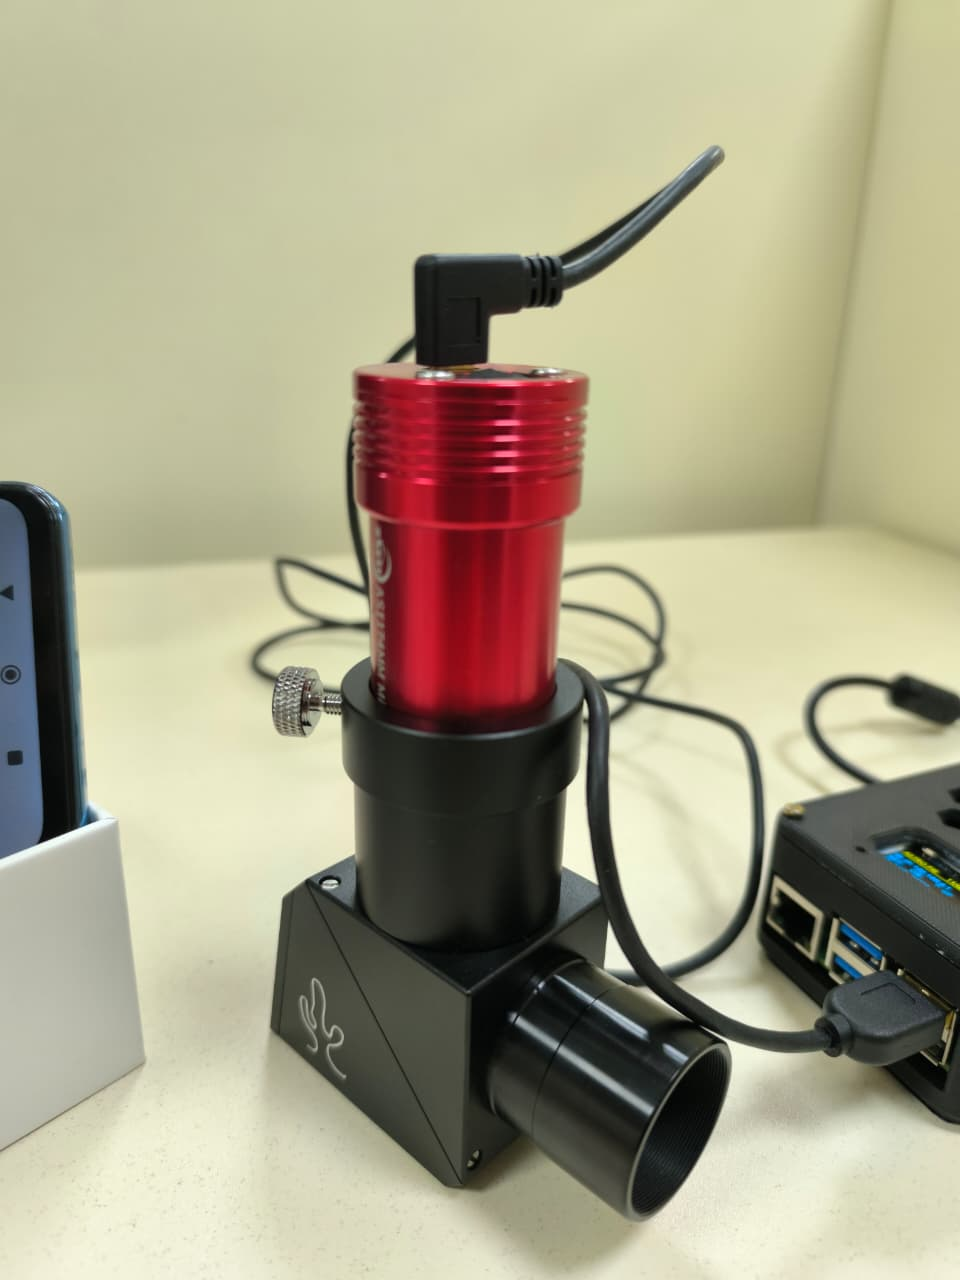
\includegraphics[width=\textwidth]{figures/hw/mount.jpeg}
        \caption{Montaje de la cámara ZWO ASI174MM Mini con el filtro Herschel.}
    \end{subfigure}
    \hfill
    \begin{subfigure}[t]{0.47\textwidth}
        \centering
        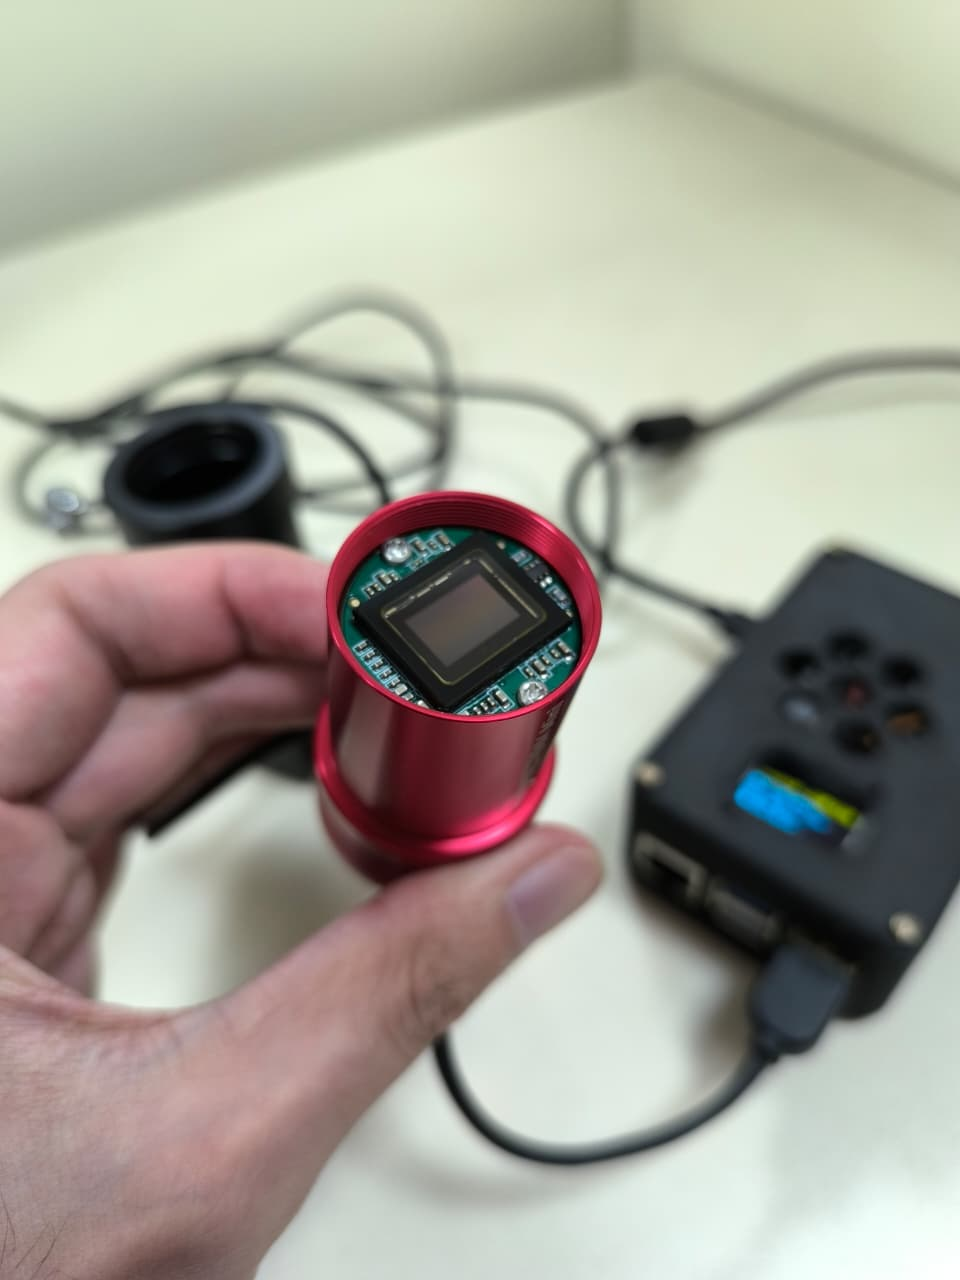
\includegraphics[width=\textwidth]{figures/hw/sensor.jpeg}
        \caption{Vista del sensor monocromático empleado para la adquisición.}
    \end{subfigure}
    \caption{Bloque de adquisición óptica empleado en la validación. Se muestran
    (a) el acoplamiento de la cámara con el filtro de atenuación solar y (b) el
    detalle del sensor de la cámara ZWO utilizado para la captura en luz blanca. \textbf{Fuente:} Elaboración propia.}
    \label{fig:camara-filtro-sensor-validacion}
\end{figure}

\begin{figure}[H]
    \centering
    \begin{subfigure}[t]{0.35\textwidth}
        \centering
        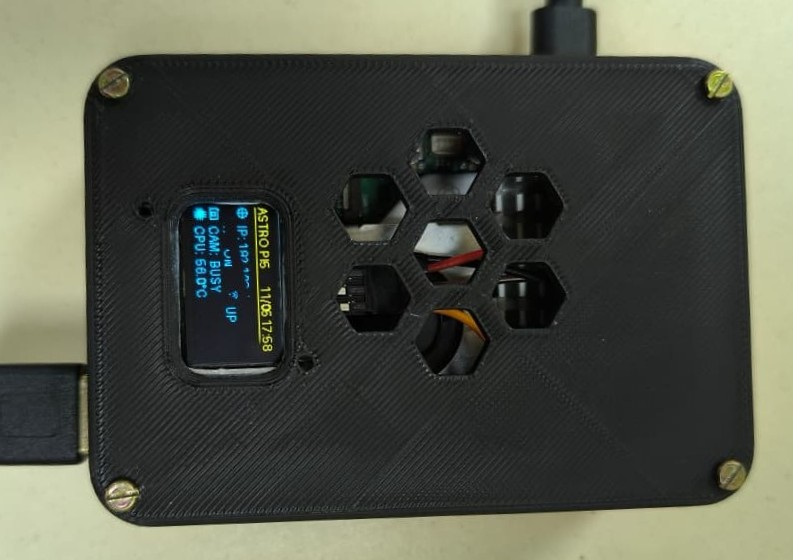
\includegraphics[width=\textwidth]{figures/hw/obs_module.jpeg}
        \caption{Módulo de preprocesamiento empleado durante las pruebas.}
    \end{subfigure}
    \hfill
    \begin{subfigure}[t]{0.6\textwidth}
        \centering
        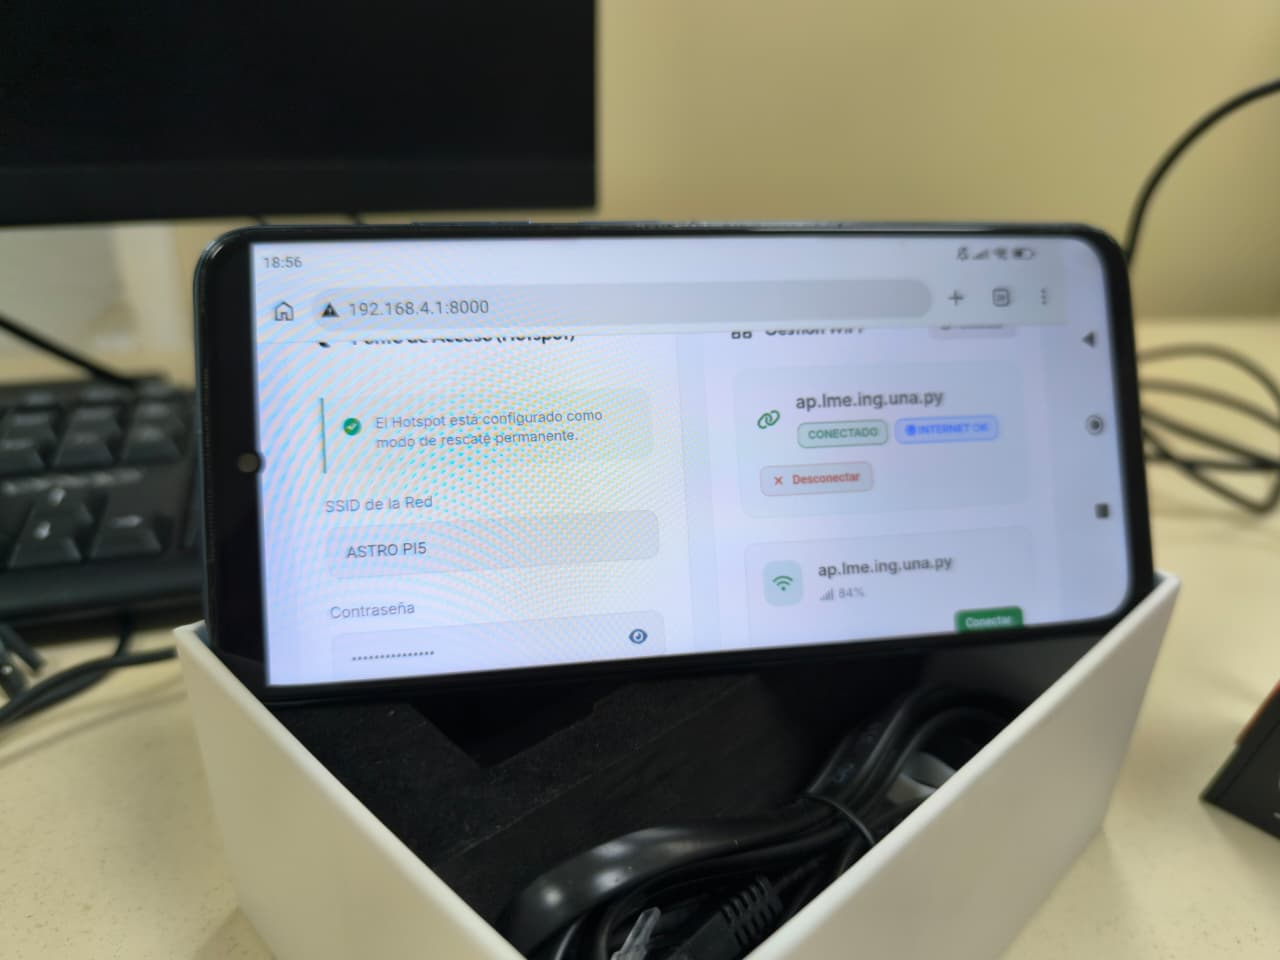
\includegraphics[width=\textwidth]{figures/hw/panel.jpeg}
        \caption{Acceso al panel local desde un dispositivo móvil.}
    \end{subfigure}
    \caption{Operación local de la unidad de preprocesamiento. Se muestran (a)
    el panel de control utilizado para supervisar el sistema y (b) el módulo
    desarrollado para integrar adquisición, preprocesamiento y conectividad. \textbf{Fuente:} Elaboración propia.}
    \label{fig:telefono-modulo-preprocesamiento-validacion}
\end{figure}

\begin{figure}[H]
    \centering
    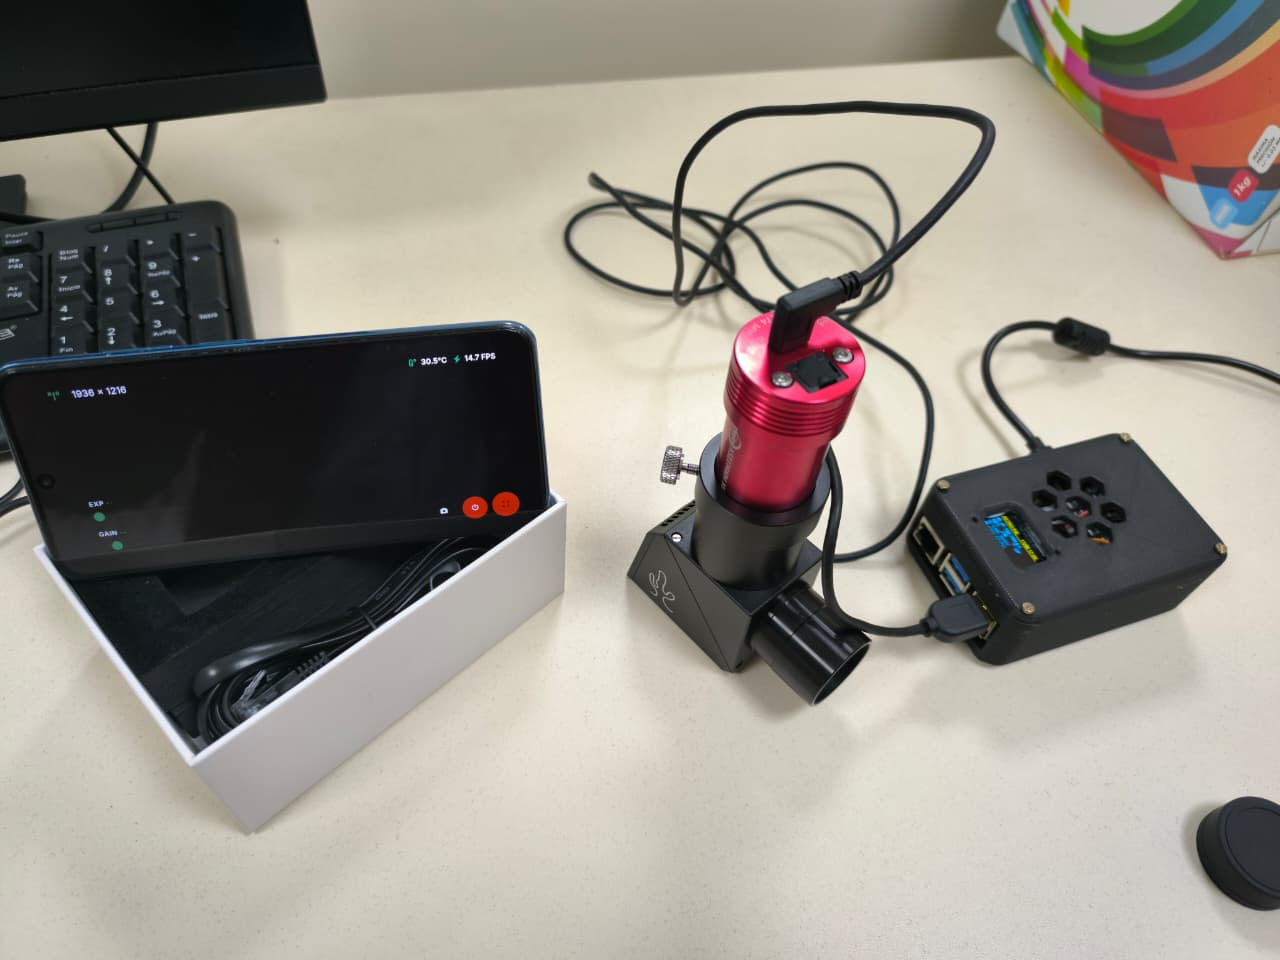
\includegraphics[width=0.72\textwidth]{figures/hw/integrated.jpeg}
    \caption{Hardware integrado del prototipo durante la etapa de validación,
    incluyendo la unidad de procesamiento local y los periféricos asociados. \textbf{Fuente:} Elaboración propia.}
    \label{fig:hardware-integrado-validacion}
\end{figure}

\begin{figure}[H]
    \centering
    \begin{subfigure}[t]{0.35\textwidth}
        \centering
        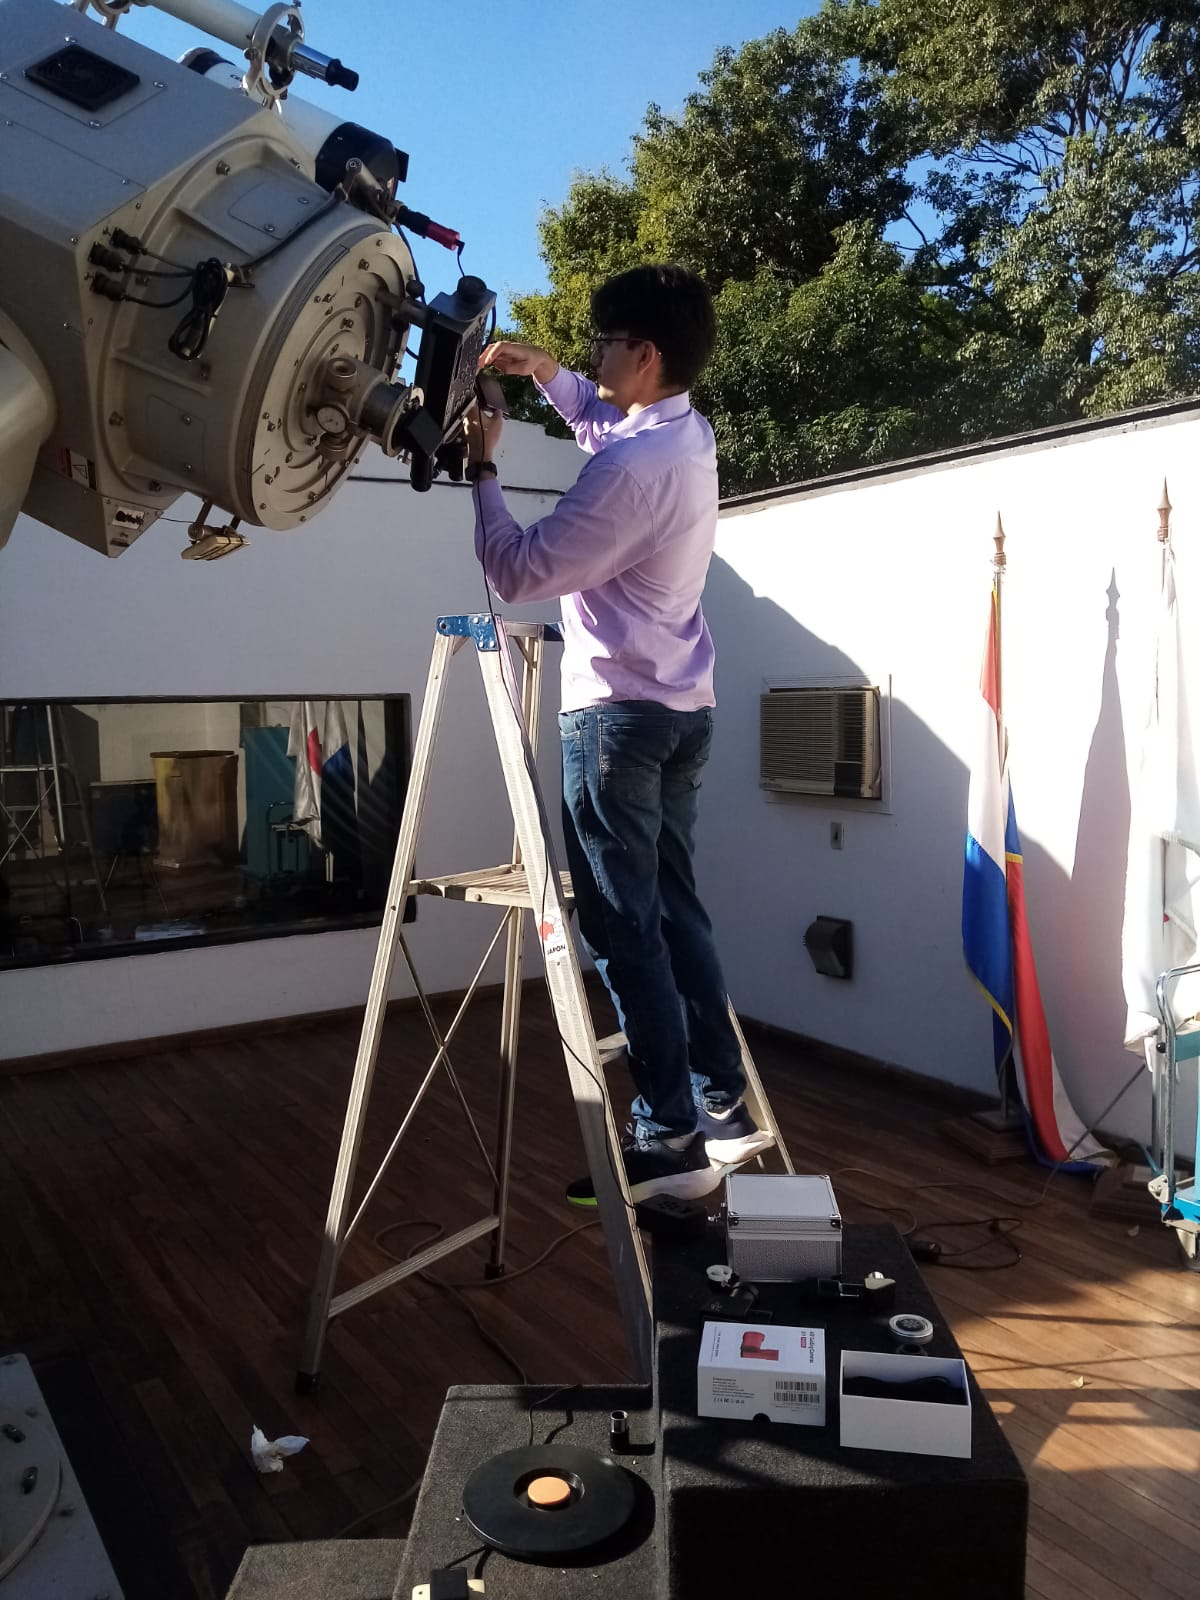
\includegraphics[width=\textwidth]{figures/hw/telescope.jpg}
        \caption{Telescopio del observatorio utilizado para las pruebas.}
    \end{subfigure}
    \hfill
    \begin{subfigure}[t]{0.6\textwidth}
        \centering
        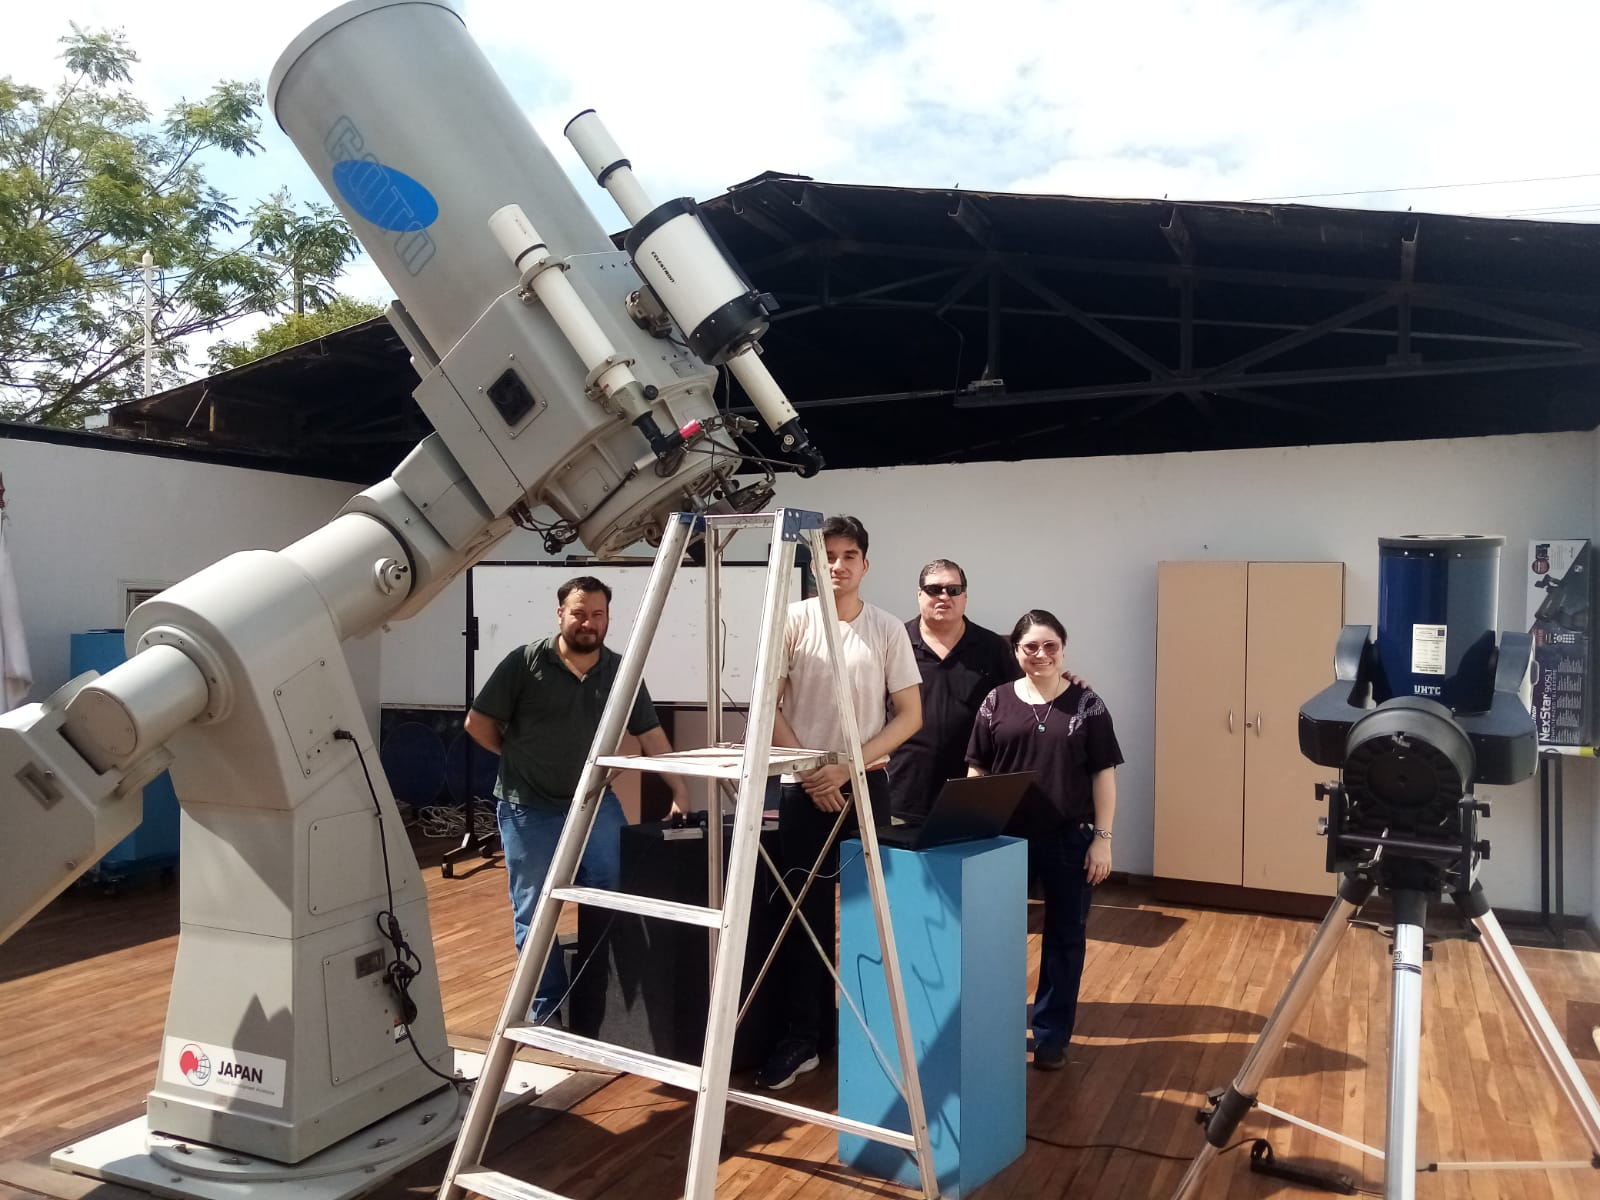
\includegraphics[width=\textwidth]{figures/hw/telescope_team.jpg}
        \caption{Integración del prototipo con el telescopio.}
    \end{subfigure}
    \caption{Integración del hardware con el telescopio del observatorio. Se
    muestran (a) el instrumento empleado para las pruebas y (b) el conjunto
    instalado para la validación del sistema completo. \textbf{Fuente:} Elaboración propia.}
    \label{fig:telescopio-integracion-validacion}
\end{figure}

\subsection{Métricas operativas en Raspberry Pi 5}

Además de verificar la integración física, se documentó una captura real
realizada el 2026-05-05 con el telescopio y el hardware de adquisición del
prototipo. La sesión se realizó bajo condiciones climáticas óptimas, con cielo
totalmente despejado, lo que favoreció la estabilidad de iluminación y la nitidez
de las capturas. Las imágenes resultantes fueron almacenadas en la base de datos
como parte del flujo operativo del sistema, permitiendo validar no solo la
obtención de la imagen, sino también su persistencia dentro de la infraestructura
de registro.

\begin{figure}[H]
    \centering
    \begin{subfigure}[t]{0.48\textwidth}
        \centering
        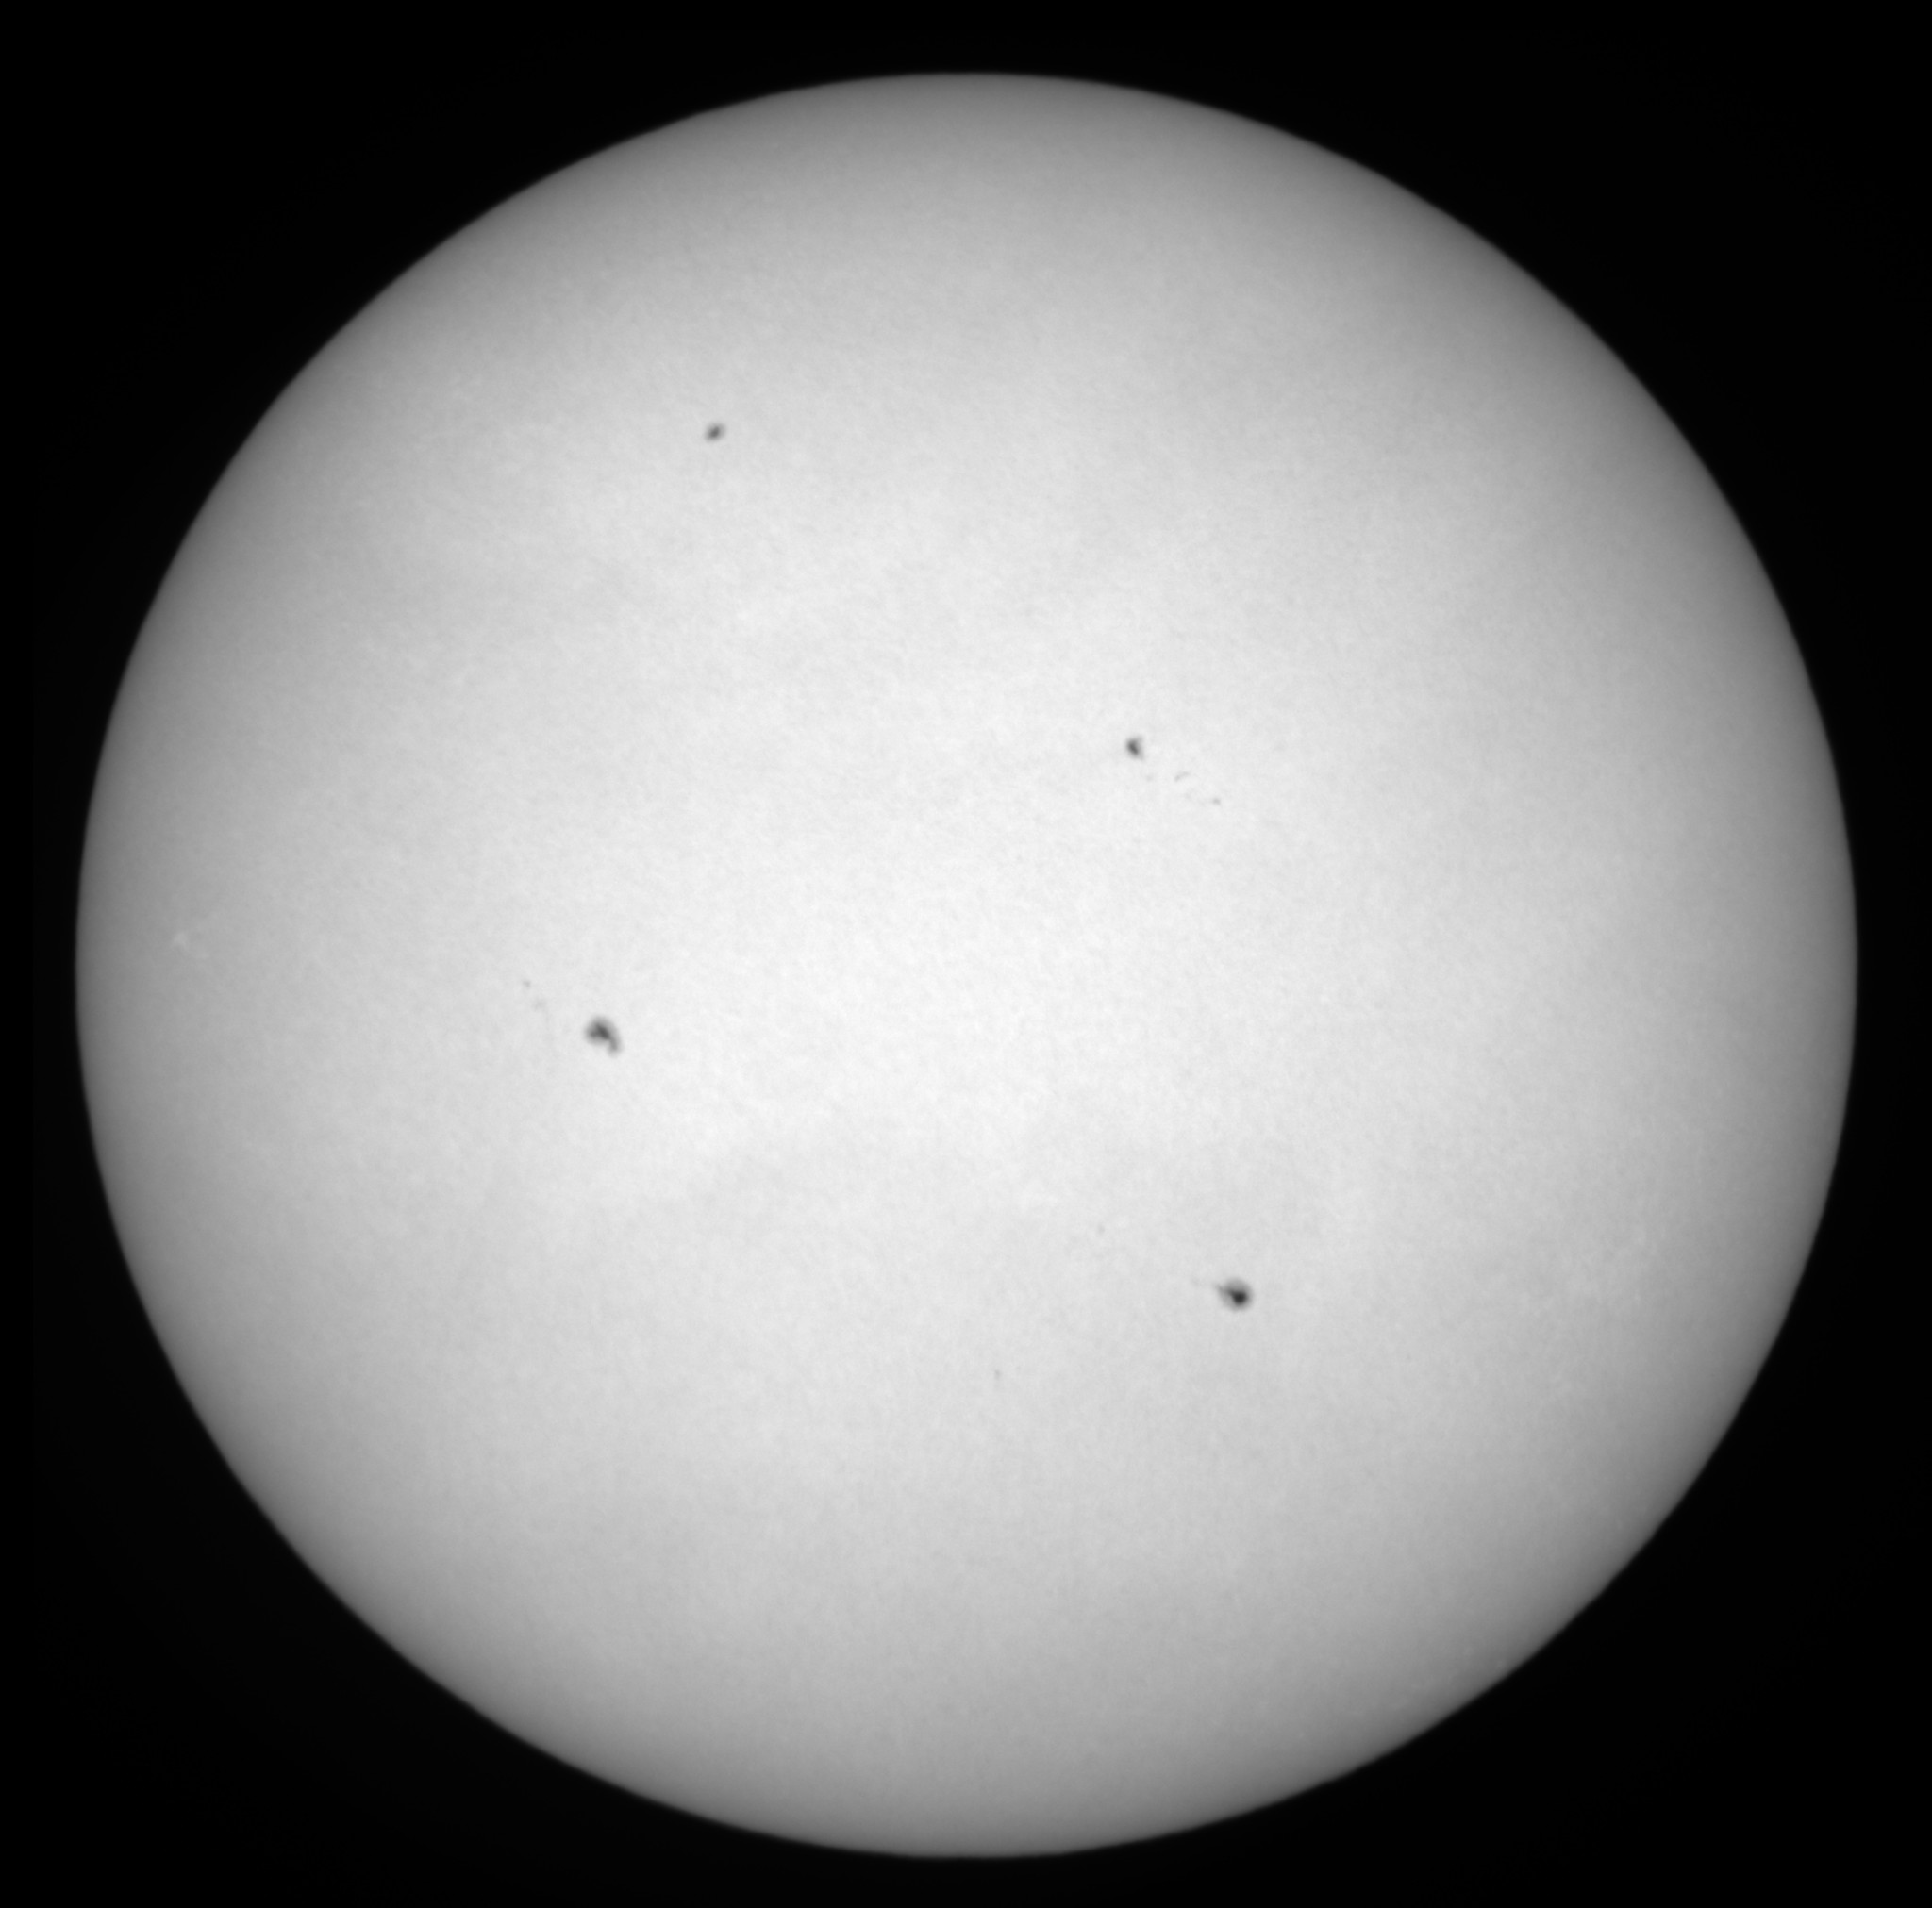
\includegraphics[width=\textwidth]{figures/obs/capture.jpg}
        \caption{Captura solar registrada durante la sesión del 2026-05-05.}
    \end{subfigure}
    \hfill
    \begin{subfigure}[t]{0.48\textwidth}
        \centering
        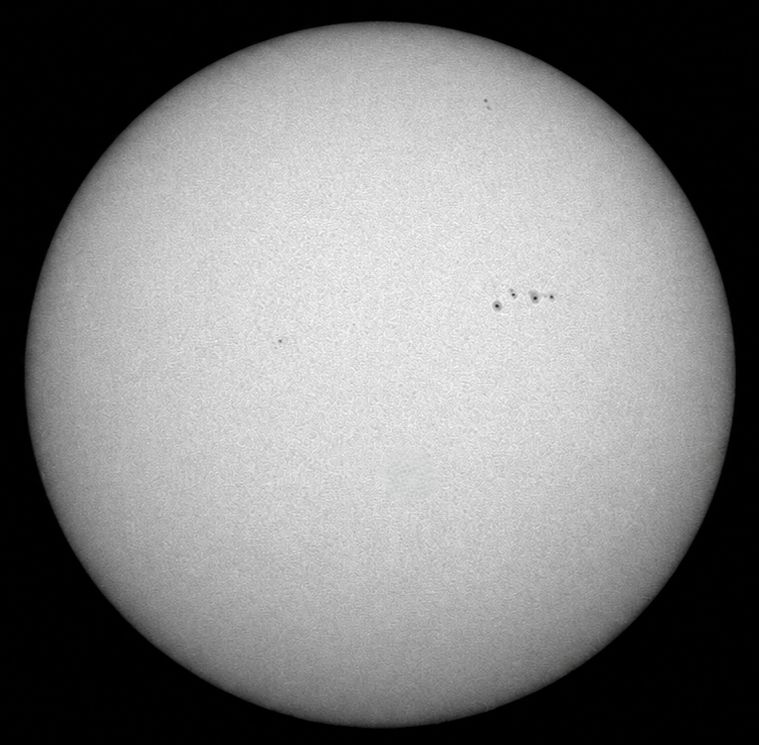
\includegraphics[width=\textwidth]{figures/obs/site.jpg}
        \caption{Imagen solar registrada el 20-05-2026 y almacenada en la base de datos del sistema.}
    \end{subfigure}
    \caption{Imágenes solares obtenidas mediante el telescopio y el hardware de
    adquisición del prototipo. \textbf{Fuente:} Elaboración propia.}
    \label{fig:capturas-solares-20260505-validacion}
\end{figure}

La Tabla~\ref{tab:parametros-captura-20260505} resume los parámetros de ajuste
empleados durante esta captura. La denominación \texttt{pi5-observatory}
corresponde al panel de interacción ejecutado en el servidor local de la
Raspberry Pi 5, desde el cual se controlan los parámetros de adquisición y se
coordina el registro de las observaciones.

\begin{table}[H]
\centering
\caption{Parámetros de adquisición utilizados durante la captura solar del
2026-05-05. \textbf{Fuente:} Elaboración propia.}
\label{tab:parametros-captura-20260505}
\uniformtablestyle
\begin{tabular}{ll}
\toprule
\textbf{Parámetro} & \textbf{Valor} \\
\midrule
Aplicación local & pi5-observatory \\
Versión & 1.0 \\
FPS & 15 \\
Temperatura del sensor & 36.7 °C \\
Binning & 1 \\
Ganancia & 1 \\
Ancho de imagen & 1936 px \\
Alto de imagen & 1216 px \\
Exposición & 500 us \\
\bottomrule
\end{tabular}
\end{table}

Además de esta evidencia de captura, se registraron métricas operativas de la
Raspberry Pi 5 durante sesiones típicas de adquisición, almacenamiento local y
sincronización remota. La Tabla~\ref{tab:metricas-raspberry-operacion} resume
valores representativos obtenidos con refrigeración activa, cámara ZWO ASI174MM
Mini y conexión WiFi disponible. Los tiempos de sincronización dependen del ancho
de banda efectivo, por lo que deben interpretarse como referencia de operación y
no como límite absoluto del sistema.

\begin{table}[H]
\centering
\caption{Métricas de rendimiento operativo del nodo Raspberry Pi 5 durante una sesión típica. \textbf{Fuente:} Elaboración propia.}
\label{tab:metricas-raspberry-operacion}
{\uniformtablestyle
\begin{tabular}{lc}
\toprule
\textbf{Métrica} & \textbf{Valor representativo} \\
\midrule
Tiempo de captura de imagen individual & 420 ms \\
Guardado local en almacenamiento microSD & 180 ms \\
Captura + guardado local & 600 ms \\
Preprocesamiento básico por imagen & 1350 ms \\
Sincronización a Supabase & 3800 ms/imagen \\
Uso medio de CPU en operación típica & 38\% \\
Uso máximo de CPU durante preprocesamiento & 72\% \\
Uso de RAM del servicio local & 3.3 GB \\
Temperatura tras sesión de 25 min & 57 °C \\
\bottomrule
\end{tabular}
}
\end{table}

Durante las pruebas no se observaron reinicios, cierres del servicio ni
reducción térmica perceptible bajo refrigeración activa. La temperatura se
mantuvo por debajo de umbrales críticos para la Raspberry Pi 5 y el uso de RAM
quedó dentro del margen disponible del modelo de 8 GB. Estos resultados respaldan
la viabilidad de operar el prototipo como nodo local de captura y asistencia,
siempre que se mantenga ventilación adecuada y se considere la variabilidad de la
red en la etapa de sincronización.

\subsection{Validación de la plataforma web}

Posteriormente, se verificó la operación desde la plataforma web actualizada. La
validación se concentró en el rendimiento percibido durante la carga de modelos,
la consulta de datos desde Supabase y la inferencia \textit{on-device} de los
módulos de agrupamiento y clasificación. Las capturas principales incluidas en
esta sección documentan las etapas funcionales del procesamiento y de la
visualización predictiva; las pantallas auxiliares de acceso, inicio y carga se
presentan como material complementario en el Anexo~\ref{anexo:suplementario}.

Para validar el flujo de inferencia visual en la plataforma, se empleó como caso
de prueba la imagen mostrada en la Figura~\ref{fig:capturas-solares-20260505-validacion}(b),
correspondiente a una captura solar del 2026-05-05 obtenida con el telescopio y
el hardware del prototipo, y posteriormente extraída desde la base de datos. A
partir de esta imagen se ejecutaron las etapas de agrupamiento y clasificación
\textit{on-device}, cuyos resultados se muestran en las Figuras~\ref{fig:web-yolo-validacion}
y~\ref{fig:web-convnextv2-validacion}.

\begin{figure}[H]
    \centering
    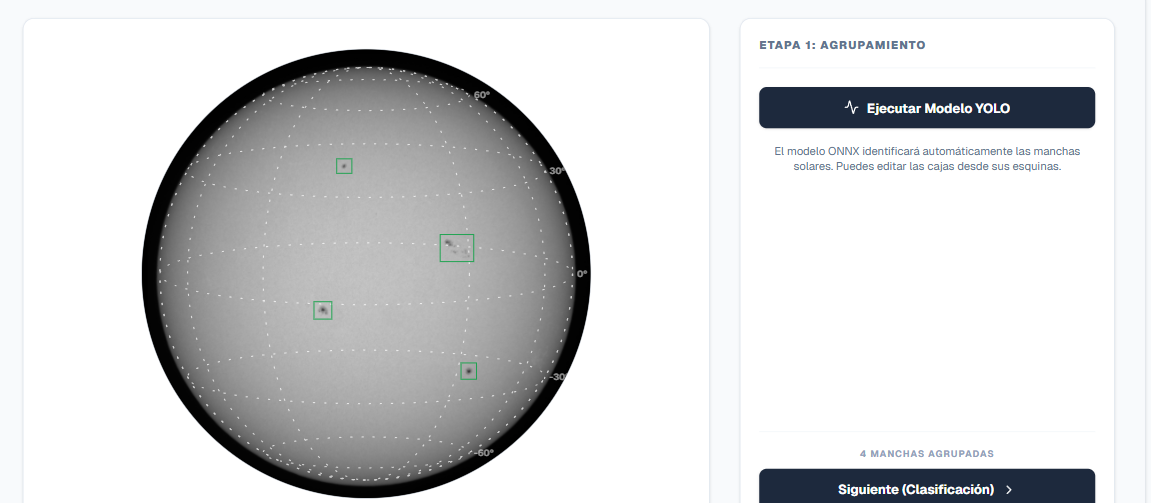
\includegraphics[width=0.82\textwidth]{figures/web/yolo.png}
    \caption{Etapa de agrupamiento \textit{on-device} aplicada a la imagen solar
    de la Figura~\ref{fig:capturas-solares-20260505-validacion}(b) mediante el
    modelo YOLO desplegado en la plataforma web. \textbf{Fuente:} Elaboración propia.}
    \label{fig:web-yolo-validacion}
\end{figure}

\begin{figure}[H]
    \centering
    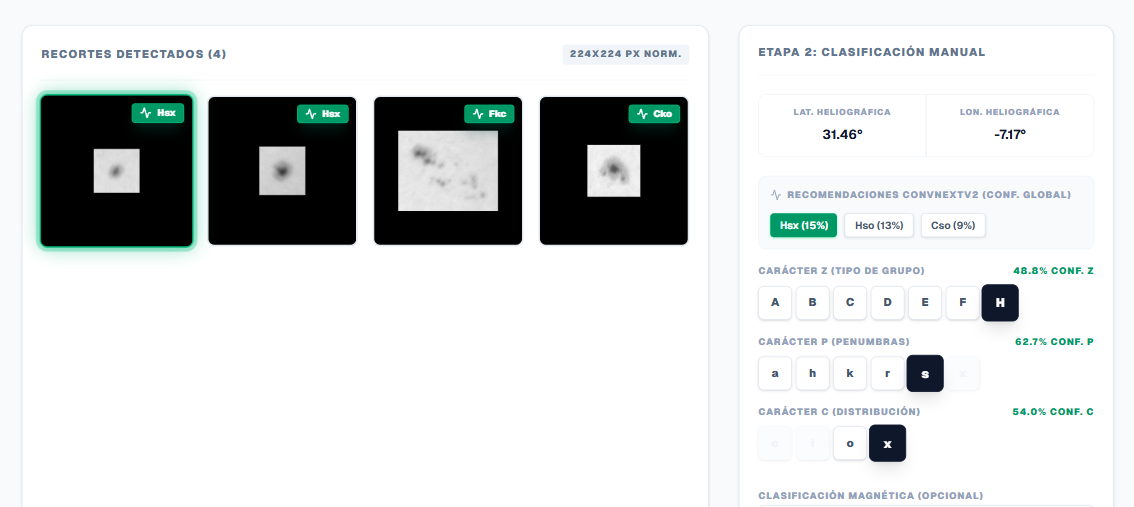
\includegraphics[width=0.82\textwidth]{figures/web/convnext.png}
    \caption{Etapa de clasificación morfológica \textit{on-device} aplicada a
    la imagen solar de la Figura~\ref{fig:capturas-solares-20260505-validacion}(b)
    mediante ConvNeXtV2 dentro de la plataforma web. \textbf{Fuente:} Elaboración propia.}
    \label{fig:web-convnextv2-validacion}
\end{figure}

\begin{table}[H]
\centering
\caption{Resultados de rendimiento de la plataforma web ejecutada en una
computadora personal. \textbf{Fuente:} Elaboración propia.}
\label{tab:rendimiento-plataforma-web-pc}
\uniformtablestyle
\begin{tabular}{ll}
\toprule
\textbf{Métrica} & \textbf{Valor} \\
\midrule
Dispositivo & Laptop ASUS TUF Gaming F15 \\
CPU & 12th Gen Intel(R) Core(TM) i5-12500H (2.50 GHz) \\
Núcleos simulados & 16 \\
CPU throttling & Nativo \\
Modo de red & Fibra / nativo \\
Velocidad de red & 780.0 Mbps / 585.0 Mbps \\
Proveedor de ejecución & \texttt{executionProviders: ["wasm"]} \\
Tiempo de descarga del modelo & 5803 ms \\
Tiempo de galería Supabase & 1702 ms \\
Inferencia YOLO & 3105 ms \\
Inferencia de clasificación & 3201 ms \\
\bottomrule
\end{tabular}
\end{table}

Aunque el equipo de prueba dispone de una GPU NVIDIA GeForce RTX 3050 Laptop GPU
de 4 GB y de gráficos integrados Intel(R) Iris(R) Xe Graphics de 128 MB, la
ejecución de los modelos se condicionó al proveedor \texttt{wasm}. Esta decisión
evita utilizar aceleración por GPU durante la inferencia y permite aproximar el
comportamiento esperado en dispositivos de recursos más limitados, donde el
procesamiento debe sostenerse principalmente mediante CPU y WebAssembly.

Además del procesamiento visual, la plataforma integra módulos predictivos para
consultar la evolución temporal del número de manchas solares y la distribución
latitudinal de la actividad. Estos módulos no operan sobre una captura individual,
sino sobre series históricas y reconstrucciones espacio-temporales, por lo que
complementan la clasificación morfológica con una lectura de tendencia solar.

\begin{figure}[H]
    \centering
    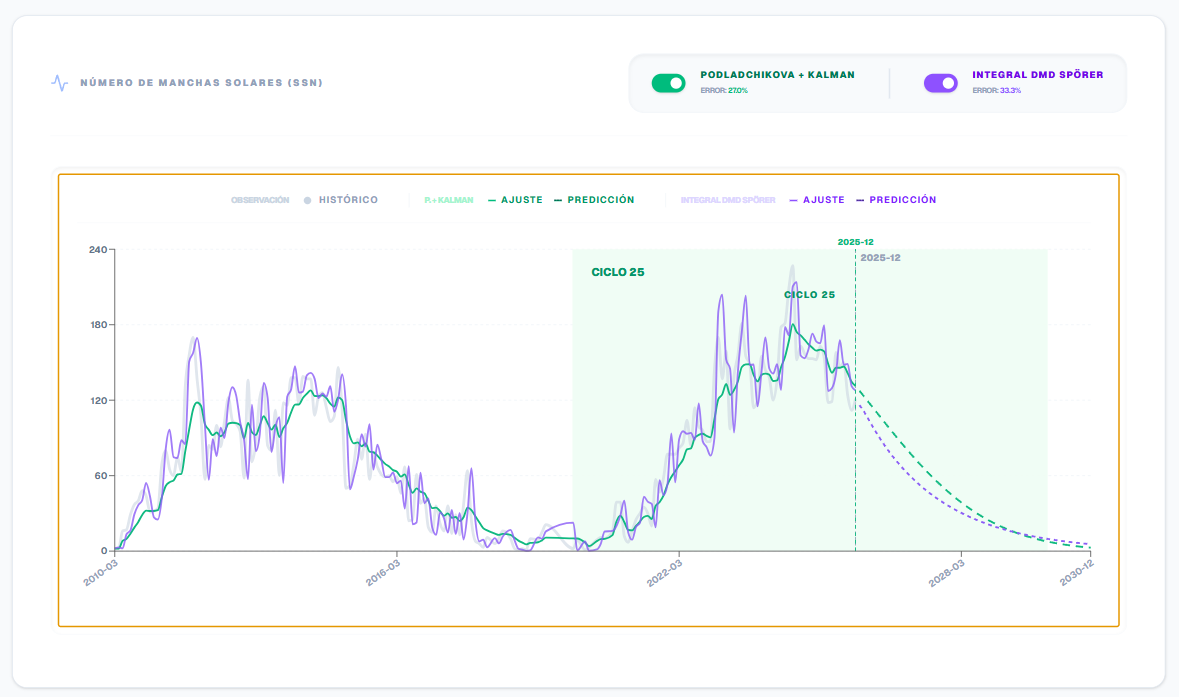
\includegraphics[width=0.82\textwidth]{figures/web/ssn.png}
    \caption{Módulo de predicción temporal del número de manchas solares
    integrado en la plataforma web. \textbf{Fuente:} Elaboración propia.}
    \label{fig:web-ssn-prediccion-validacion}
\end{figure}

\begin{figure}[H]
    \centering
    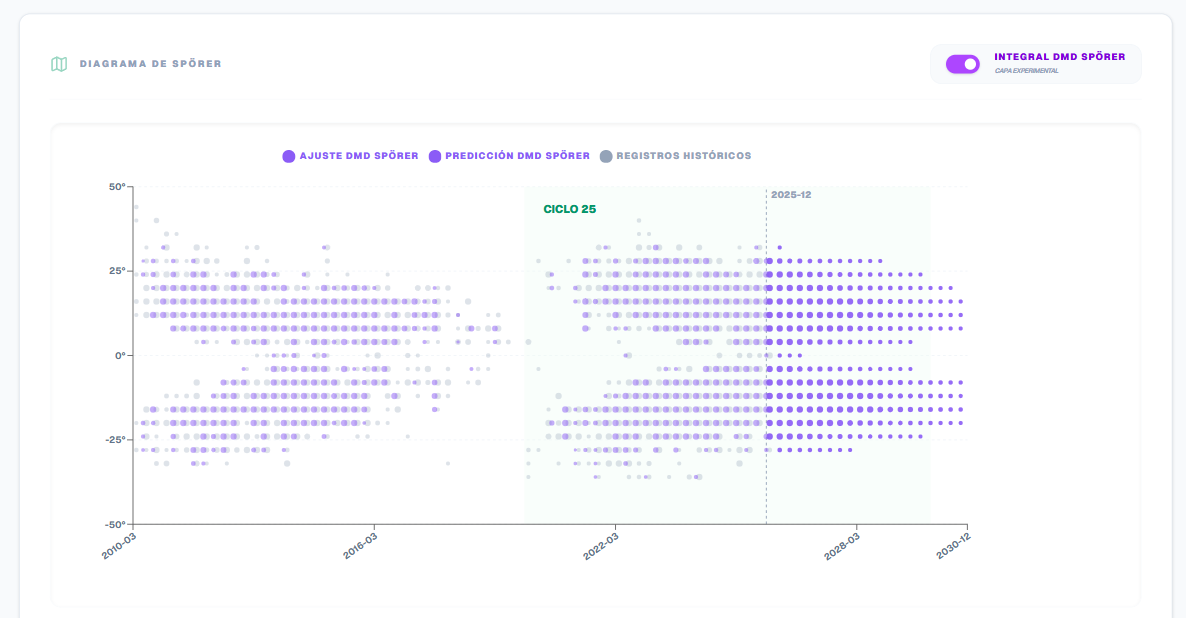
\includegraphics[width=0.82\textwidth]{figures/web/butterfly.png}
    \caption{Visualización del diagrama de mariposa para analizar la
    distribución latitudinal de la actividad solar. \textbf{Fuente:} Elaboración propia.}
    \label{fig:web-diagrama-mariposa-validacion}
\end{figure}

En términos funcionales, la validación confirma que el sistema puede capturar
imágenes, registrar metadatos, ejecutar inferencia local mediante modelos ONNX
y almacenar los resultados en la base de datos sin intervención manual
significativa. Los modelos ONNX exportados pesan en conjunto aproximadamente
24~MB, un tamaño adecuado para descarga, sincronización y actualización en
entornos de conectividad limitada. Esta evidencia respalda la consistencia
operativa del prototipo y demuestra que la solución propuesta trasciende el
entrenamiento aislado de modelos para constituirse en una plataforma de
asistencia observacional integrada.


\section{Análisis de Costos e Inversión del Proyecto}

La implementación del prototipo requirió una inversión directa asociada a los
componentes principales de adquisición, atenuación óptica, procesamiento local,
visualización de estado y soporte físico. La Tabla~\ref{tab:presupuesto-prototipo}
resume el presupuesto referencial empleado para construir la configuración
validada.

\begin{table}[H]
\centering
\caption{Presupuesto referencial de componentes principales del prototipo. Los montos en guaraníes se estiman con un tipo de cambio referencial de 1 USD = 6108 PYG. \textbf{Fuente:} Elaboración propia.}
\label{tab:presupuesto-prototipo}
\uniformtablestyle
\begin{tabularx}{\textwidth}{>{\raggedright\arraybackslash}X r r}
\toprule
\textbf{Componente} & \textbf{Precio USD} & \textbf{Precio PYG} \\
\midrule
Raspberry Pi 5 8 GB & 190 & 1160520 \\
Módulo active cooler para Raspberry Pi 5 & 13 & 79404 \\
Cámara ZWO ASI174MM Mini & 432 & 2638656 \\
Filtro solar Herschel wedge Lunt 1.25'' con ND3 & 308 & 1881264 \\
Pantalla OLED 0.96'' 128x64 & 9 & 54972 \\
Impresión 3D de carcasa y soporte & 4 & 24432 \\
\midrule
\textbf{Total} & \textbf{956} & \textbf{5839248} \\
\bottomrule
\end{tabularx}

\end{table}

El costo total estimado del prototipo fue de US\$956, equivalente a
5,839,248 PYG bajo el tipo de cambio referencial utilizado en la tabla. Este
monto incluye los elementos indispensables para disponer de una estación local de
captura solar en luz blanca: unidad de procesamiento, refrigeración, cámara,
cuña de Herschel, pantalla de estado y soporte impreso en 3D. La mayor parte de
la inversión se concentra en la cámara monocromática y el sistema de atenuación
solar, componentes críticos para preservar calidad de imagen y seguridad óptica.

El proyecto fue financiado parcialmente por el programa de becas PUBIABM, que
cubrió el 70\% del costo total del prototipo. Este esquema de financiamiento permitió reducir la carga económica
directa de implementación y facilitó la adquisición de componentes de mayor
impacto técnico sin comprometer la reproducibilidad del sistema.

Desde el punto de vista de inversión, el prototipo mantiene una relación
favorable entre costo y funcionalidad. La selección de Raspberry Pi 5 evita
recurrir a estaciones de trabajo dedicadas para la etapa de captura; el uso de
software abierto y modelos exportados a ONNX reduce dependencias de licencias o
servidores de inferencia; y la carcasa impresa en 3D disminuye costos de
integración mecánica. Además, varios componentes pueden reutilizarse en futuras
campañas observacionales o en extensiones del sistema, por lo que la inversión no
se limita a una única sesión de validación. Al finalizar el trabajo, todos los
elementos adquiridos serán donados al Observatorio Astronómico ``Prof.~Alexis
Troche Boggino'', de modo que queden disponibles para continuidad operativa,
formación académica y otros proyectos afines de observación solar o desarrollo
instrumental.

\section{Limitaciones de la validación actual}

Aunque los resultados obtenidos son consistentes con los objetivos del trabajo,
la validación presenta algunas restricciones. La principal limitación radica en el
tamaño y distribución de los conjuntos de datos, especialmente en clases poco
frecuentes de la taxonomía Zurich--McIntosh. Asimismo, la evaluación en campo
se realizó sobre un número acotado de sesiones observacionales y bajo una
configuración instrumental específica. Esta restricción se ve reforzada por el
hecho de que las observaciones óptimas dependen de condiciones climáticas
favorables, cuya variabilidad dificulta significativamente la adquisición, y por
el rango horario limitado en el que el Sol es observable desde el observatorio.

Por otra parte, los modelos predictivos deben interpretarse como herramientas
de apoyo para el análisis exploratorio y no como sistemas operacionales de
pronóstico solar. Su utilidad principal radica en complementar la interpretación
temporal de la actividad observada.

Estas limitaciones no invalidan los resultados presentados, pero delimitan el
alcance de las conclusiones y señalan oportunidades claras para trabajos
futuros orientados a ampliar la base de datos, incorporar observaciones
adicionales y refinar los modelos desarrollados.